\chapter{Semantic Tag Sets}
Semantic tags can stored together in a set. Each Shark set behaves like Java sets typically do: Tags can be added and removed. 

Tags can have relations. Relations can only be defined by means of tag 
sets. From that structural point of view, Shark offers three kind of sets:

\begin{description}
\item[ST Sets] are also called {\it plain sets}. The just store tags. Tags don't have any additional relation.
\item[Taxonomy] also stores tags. {\tt TXSemanticTags} can be in a hierarchical 
relations, e.g. tag A is {\tt sub} topic of tag B and tag B is {\tt super} topic of A in that case.
\item[SemanticNet] also store tags. {\tt SNSemanticTags} can have arbitrary relations. Relations are usually illustrated by an arc. One tag can refer another tag with a {\tt predicate}\footnote{Yes, this terminology is taken from W3C RDF. The Shark model is far less complex, though.}.
\end{description}

\section{Create, Merge, Add, Remove}
The following code sample creates a plain tag set. A semantic tag is created and removed afterwards.

\begin{verbatim}
STSet plainSet  = InMemoSharkKB.createInMemoSTSet();

SemanticTag berlin = 
   plainSet.createSemanticTag("Berlin", "http://www.berlin.de");

plainSet.removeSemanticTag(berlin);
\end{verbatim}

That's a good point to discuss relationship between knowledge base, sets and 
tags. Tags can either be part of a tag set or exist alone in memory.

There are several knowledge base implementations which will be discussed later in this book. The {\verb|InMemoSharkKB|} exists only in computer memory. All other implementations persist their data on an external medium.

Semantic Tags {\bf cannot} be moved from one set to another. A tag remains in the environment where it was created. A tag that was created remains in memory. A tag that was created in a tag set remains their until its deletion. 

Tags and sets can be {\bf merged}, though. Merging means creating a copy.
Tags can be merged into a set. Sets can be merged into other sets.

Moving a tag from one set two another could be implemented as two step algorithm: First, merge the tag to the target set. Second, remove it from source set. This algorithm behave as moving only if the target set does not contain an {\it identical} tag. This becomes - hopefully - clear when having a look on the merging algorithm:

First, it is looked for
an identical tag inside the set. If there is one, both tags are merged. A copy of the tag is added otherwise. Note: Properties are copied as well, regardless if they are defined to be transferable or not.

Merging tag sets works similar. All tags from the source set are iterated and merged into the target set.

The following code illustrates some examples.

\begin{verbatim}
// create a semantic tag in memory
SemanticTag paris = InMemoSharkKB.createInMemoSemanticTag(
   "Paris", "http://www.paris.fr");

// create stand alone set in memory
STSet plainSet  = InMemoSharkKB.createInMemoSTSet();

// create tag inside tags a tag set
SemanticTag berlin = plainSet.createSemanticTag(
   "Berlin", "http://www.berlin.de");

// merge a tag into a tag set
SemanticTag parisCopy = plainSet.merge(paris);

// create a kb instance
InMemoSharkKB kb = new InMemoSharkKB();

// get the already created set of topics which is still empty 
STSet topicSTSet = kb.getTopicSTSet();

// merge the berlin and paris tag into the knowledge base
topicSTSet.merge(plainSet);
\end{verbatim}

\section{SemanticNet}
Semantic tags can have relations. More precisely, semantic tags can represent things which have relations. Let's have an example.

A tag might describe Germany. Another tag might describe Berlin which is a city in Germany. We'd like to describe that fact.

\begin{figure}[t]
\centering
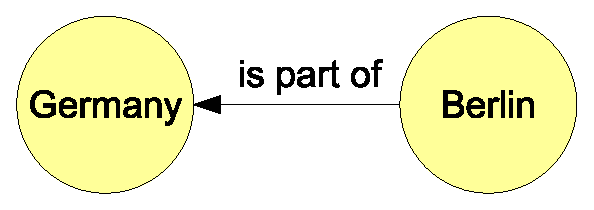
\includegraphics[width=0.40\textwidth]{semanticNet.eps}
\caption{A little semantic net}
\label{fig:semanticNet}
\end{figure}

Tags can refer to another tag by a {\it predicate}. A predicate has two parameters: the referred tag ({\it target} and the predicate name. The origin of the predicate is called {\it source}. 

For our example, the {\it Berlin} tag could refer to the tag {\it Germany} with a predicate named {\it is part of}, see figure \ref{fig:semanticNet}

The following code creates that data structure in memory.

\begin{verbatim}
public class SemanticNetSample {
  public static void main(String args[]) throws SharkKBException {
    SharkKB kb = new InMemoSharkKB();
        
    // handle topics as semantic net
    SemanticNet sn = kb.getTopicsAsSemanticNet();
        
    // describe Germany
    SNSemanticTag germany = sn.createSemanticTag("Germany", 
    "http://en.wikipedia.org/wiki/Germany");
        
    // describe Berlin
    SNSemanticTag berlin = sn.createSemanticTag("Berlin", 
    "http://en.wikipedia.org/wiki/Berlin");
        
    // define a relationname
    String isPartOf = "isPartOf";

    // define berlin to be a part of Germany
    berlin.setPredicate(isPartOf, germany);
        
    /* 
     * what parts of Germany are defined yet?
     */ 
    Enumeration<SNSemanticTag> partsEnum = 
       germany.sourceTags(isPartOf);
        
    // berlin has relations to what tags?
    Enumeration<SNSemanticTag> targetTags = 
       berlin.targetTags(isPartOf);
  }       
}

\end{verbatim}

The first line creates an in-memory knowledge base. The second line
gets a reference to the topic dimension of the knowledge base. Each dimension can be handled differently. It can be handled as plain set, as taxonomy or as semantic net as in this example.

Two tags are created, one representing Germany, another one for Berlin. The string {\it istPartOf} is defined for this application. It is just am arbitrary string! 

The line {\verb|berlin.setPredicate(isPartOf, germany)|} sets the predicate. 

{\verb|germany.sourceTags(isPartOf)|} returns an enumeration of source tags.
Remember, source tags are the start of a predicate. Thus, that method returns any tag the refers to {\tt germany} with the {\tt isPartOf} predicate.

{\verb|berlin.targetTags(isPartOf)|} returns an enumeration of target tags.
In this case, we get all tags to which {\tt berlin} is linked with the {\tt isPartOf} predicate.

Does it sound confusing? On the first glimpse it probably will. It will instantly less frustrating when you have made a little sketch by your own.

To sum up, predicates have the following features and conventions:

\begin{itemize}

\item Each tag can refer to an arbitrary number of other tags. 

\item
Each predicate name can be used in an arbitrary number of predicates.

\item
Referred tags are called {\bf target tags}. The tag that actual refers to another tag is called {\bf source tag} -- it is the source of the predicate.

\item
Predicates can be removed. It doesn't change anything in related tags.

\end{itemize}

\section{Taxonomy}
Taxonomies are special semantic nets. There are just two types of predicates:
{\it super} and {\it sub}. Taxonomies are used if semantic tags can be arranged into a hierarchy of concepts.

Taxonomies have the following features:

\begin{itemize}
    \item 
Tags can be {\it moved under} another tag which means that one tag becomes the sub-tag of another one.

    \item 
Each tag can have an arbitrary number of sub-tags but just one super-tag.

    \item 
A tag without a super-tag is called {\bf root-tag}. A taxonomy has at least one but can have more than one root tag. Our taxonomy is actually a {\it wood}.

    \item 
Tags can be removed. Sub-tags have to be handled in this case. There are two cases: If the deleted tag was a root-tag, all of its sub-tags become root-tags. If the deleted tag was a sub-tag, all of its sub-tags become sub-tags of the super-tag of the deleted tag.

\end{itemize}

Figure \ref{fig:taxonomy} illustrates a little taxonomy that describes the fact that Java and c-Sharp are programming languages.

\begin{figure}[t]
\centering
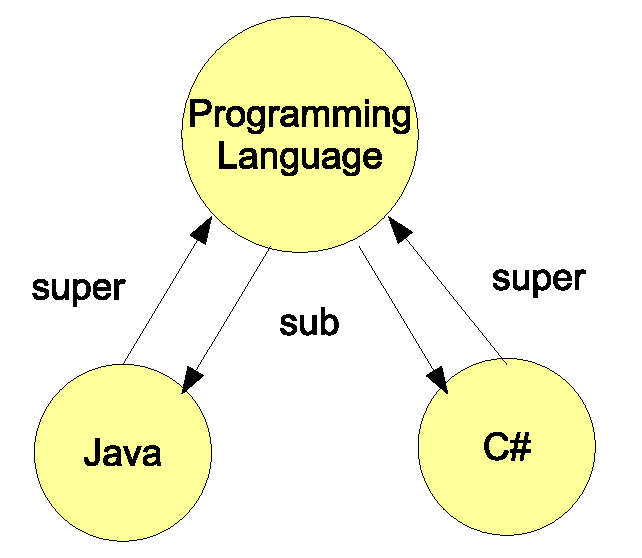
\includegraphics[width=0.40\textwidth]{taxonomy.eps}
\caption{A little taxonomy}
\label{fig:taxonomy}
\end{figure}

The following code creates a data structure representing the same fact.

\begin{verbatim}
public class TaxonomySample {
  public static void main(String args[]) throws SharkKBException {
    SharkKB kb = new InMemoSharkKB();
        
    // we are going to handle topics as taxonomy
    Taxonomy tx = kb.getTopicsAsTaxonomy();
        
    // describe programming languages and java as part of a taxonomy
    TXSemanticTag pl = 
      tx.createTXSemanticTag("PL", 
      "http://en.wikipedia.org/wiki/Programming_language");
    
    TXSemanticTag java = 
      tx.createTXSemanticTag("Java", 
      "http://en.wikipedia.org/wiki/Java_%28programming_language%29");
        
    // move java "under" pl
    java.move(pl);
        
    // describe C#
    TXSemanticTag csharp = 
      tx.createTXSemanticTag("CSharp", 
      "http://en.wikipedia.org/wiki/C_Sharp_%28programming_language%29");
        
    // define c# as sub topic of programming lanugages
    csharp.move(pl);
  }
}
\end{verbatim}

\section{Tag set operations}
Operations on semantic tag sets are actually the heart of the semantic algebra of Shark. Fragmentation and contextualization are basically defined with the tag sets. Later we learn about calculating mutual interests of different peers, extracting information from knowledge bases and assimilating knowledge. Every of those complex operations is based on the following basic operations.

\subsection{Is in}
From a logical perspective, a tag set is a disjunction (OR combination) of its tags. It can be checked whether a tag is in a set or not. Not: {\it is in} {\bf does not} mean that the actual object is in the set. {\bf It does mean} that {\it an identical tag} is in the set.

Tag set offers the {\tt isIn} method. The following code does the same job:

\begin{verbatim}
if(plainSet.getSemanticTag(paris.getSI())) != null) {
  System.out.println("is in");
}
\end{verbatim}

Remember our code from plain sets. A tag {\tt paris} was created to represent the capital of France. Tag identity is made up their subject identifier which can be retrieved with {\tt getSI()}. No, we can try to {\tt getSemanticTag} from {\tt plainSet} which is identical to {\tt paris}. 

This call succeeds if a identical tag of {\tt paris} in in {\tt plainSet}.

It is easier to write {\verb|plainSet.isIn(paris.getSI())|}

\subsection{Is any}
A tag set that only contains tags, that are defined with {\it any semantics}, are said to be an {\it any set} itself.

In other words: A set is an any set if it 

\begin{itemize}
    \item is empty or
\item
all tags have no semantics.
\end{itemize}

In all other cases a tag set is not an {\it any set}. Our Shark algebra helps again:

\begin{verbatim}
boolean isAny = SharkCSAlgebra.isAny(plainSet);
\end{verbatim}

\subsection{Identity}

Tag sets (lets call them A and B) can be identical. That's the case if for every tag in A an identical tag in B can be found and vice versa.

The definition ensures that A is not a sub set of B or vice versa. They are identical. The definition does not ensure that both sets actually contain the same Java objects. Tags can be identical without using identical memory in the computer.

Our algebra can help again:

\begin{verbatim}
boolean isIdentical = SharkCSAlgebra.identical(plainSet, plainSet2);
\end{verbatim}

\subsection{Merge}
A {\bf tag} can be merged into a set. An identical tag can already be in the set. In this case, both tags are merged (see tag merging in a previous section). Otherwise, the a copy of the tag is added to the set. The tag itself won't be changed in any case.

A {\bf set} (called {\it source}) can be merged into another set which is called {\it target set}. Each tag of the source will be merged into the target. Any relations between the tags are copied as well. After merging, the target is usually changed. The source won't be changed.

The following code first merges a single tag into a set. Second, a whole set is merged into another one.

\begin{verbatim}
plainSet.merge(paris);
plainSet.merge(plainSet2);
\end{verbatim}

Merging of sets works also with taxonomies and semantic nets. In this case, all predicates are merged as well. Such merging is a two step operation: First, all tags from the source are merged into the target with the described algorithm. Afterwards, all predicates are merged as well. 

\section{Fragmentation}
Fragmentation is one of the core algorithms in Shark. It is used in many different ways and comes in a number of different versions. We are going to discuss most of them here. It is crucial to understand that method even if it might take a while to understand the concept.

Fragmentation is a powerful tool to find out e.g. if two persons share similar interests. Fragmentation can be compared with a database query but on a semantic level.

\subsection{Plain set fragmentation}
The fragmentation operation creates a sub set from a tag set. The operation has at least two parameters: a {\it source} tag set that will be fragmented and one semantic tag called {\it anchor}. There are some variations. We start with the trivial one.

A plain tag set is just a collection of tags which are assumed to have no relations. A fragmentation is pretty simple:

During the first step, the sources tags are compared with the anchor tag. If there is no identical tag, the result of this operation is an empty tag set.

Otherwise, a tag set is created and the identical tag is merged into the newly created set.

This trivial version of fragmentation has two possible results: An empty set if the anchor is not part of the source or a set with a copy of the identical tag of anchor which is in the source.

Figure \ref{fig:simpleFragmentation} illustrates the concept.

\begin{figure}[t]
\centering
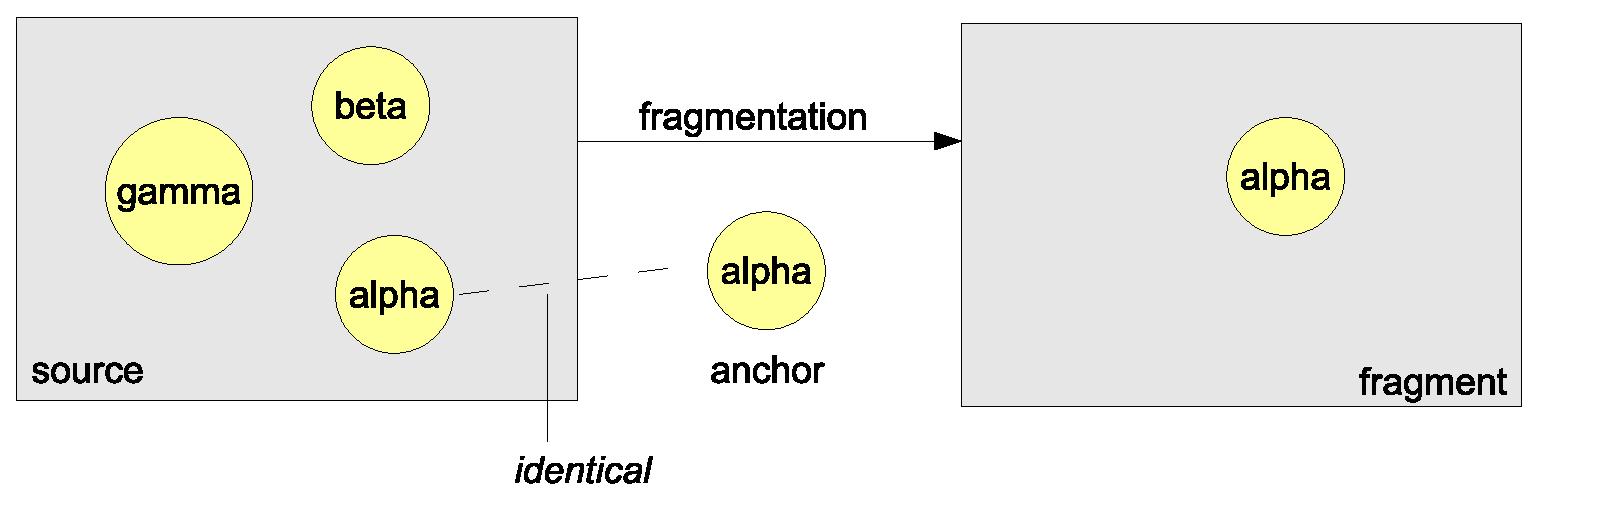
\includegraphics[width=0.60\textwidth]{simpleFragmentation.eps}
\caption{Simple fragmentation}
\label{fig:simpleFragmentation}
\end{figure}

The code constructs the source set, anchor and performs fragmentation.

\begin{verbatim}
STSet source  = InMemoSharkKB.createInMemoSTSet();

source.createSemanticTag("alpha", "http://www.alpha.de");
source.createSemanticTag("beta", "http://www.beta.de");
source.createSemanticTag("gamma", "http://www.gamma.de");

System.out.println("source:" + L.stSet2String(source));

SemanticTag anchor = 
   InMemoSharkKB.createInMemoSemanticTag(
      "alphaAnchor", "http://www.alpha.de");

System.out.println("anchor:" + L.semanticTag2String(anchor));
STSet fragment = source.fragment(anchor);

System.out.println("fragement:" + L.stSet2String(fragment));
\end{verbatim}

Run the code and see what happens. Note, the {\tt L.stSet2String} creates a string representing a set. Class {\tt L} is really useful.

\subsection{Taxonomy fragmentation}
\label{sec:taxonomyFragmentation}
Tags in taxonomies have super- and sub-relations. Therefore, the fragmentation operation has three additional parameters: {\tt depth} (a non-negative integer value) and two boolean values {\tt superAllowed} and {\tt subAllowed}.

\begin{enumerate}
    \item 
The algorithm starts like the trivial variant: The sources tags are checked for a match with the anchor tag. The algorithm stops, if no such tag can be found. 

Otherwise a new taxonomy is created and the identical tag is merged into the new taxonomy. A list of tags is created, let's call it {\it added tags}. The identical tag is stored in this list. The algorithm proceeds with the next step.

    \item 
Depth is decreased. The algorithm stops if the result is below zero.

Otherwise the {\it added tags} list is renamed to {\it current tags} and a new empty {\it added tags} list is created.

The list of {\it current tags} is iterated. The following steps are performed for every entry of the list.

    \item 
If {\tt superAllowed} is false, the next step is taken.

Otherwise, the super-tag of the current tag is taken and merged into the new taxonomy. The predicate is also copied. The super-tag is added to the {\it added tags} list.

    \item 
If {\tt subAllowed} is false, the next step is taken.

Otherwise, each sub-tag of the current tag is merged into the new taxonomy and added to the {\it added tag list}. Predicates are copied as well.

    \item 
After iterating the {\it current tags} list the algorithm continues by decreasing the depth (see above).

\end{enumerate}

Fragmentation is a kind of breadth first search. The parameter {\tt depth} defines the maximal path length from the anchor to another tag. Both logical values define if super- and/or sub-tags should be added to the fragment.

An example should help to fully understand the process. Let's assume we have a taxonomy like shown in figure \ref{fig:taxonomy} and an anchor tag, that is identical to "Tag 2" of the source tag in the picture. With a defined depth of two, {\tt subAllowed} set to {\tt true} and {\tt superAllowed} set to {\tt false}, the resulting tag set would consist of the matching "Tag 2" and all of his sub-tags of the next two layers.

Figure \ref{fig:taxonomyFragmentation} illustrates that process. Source taxonomy describes that programming languages are a part of computer science as well as
the marvelous field of semantic web. Two programming languages are mentioned.

The anchor is programming languages and the fragment is created in both directions: up to more general and down to more specific concepts. The depth is just one. The resulting fragment contains any concept (and any relation) except semantic web. which cannot be reached in one step from programming languages.

\begin{figure}[t]
\centering
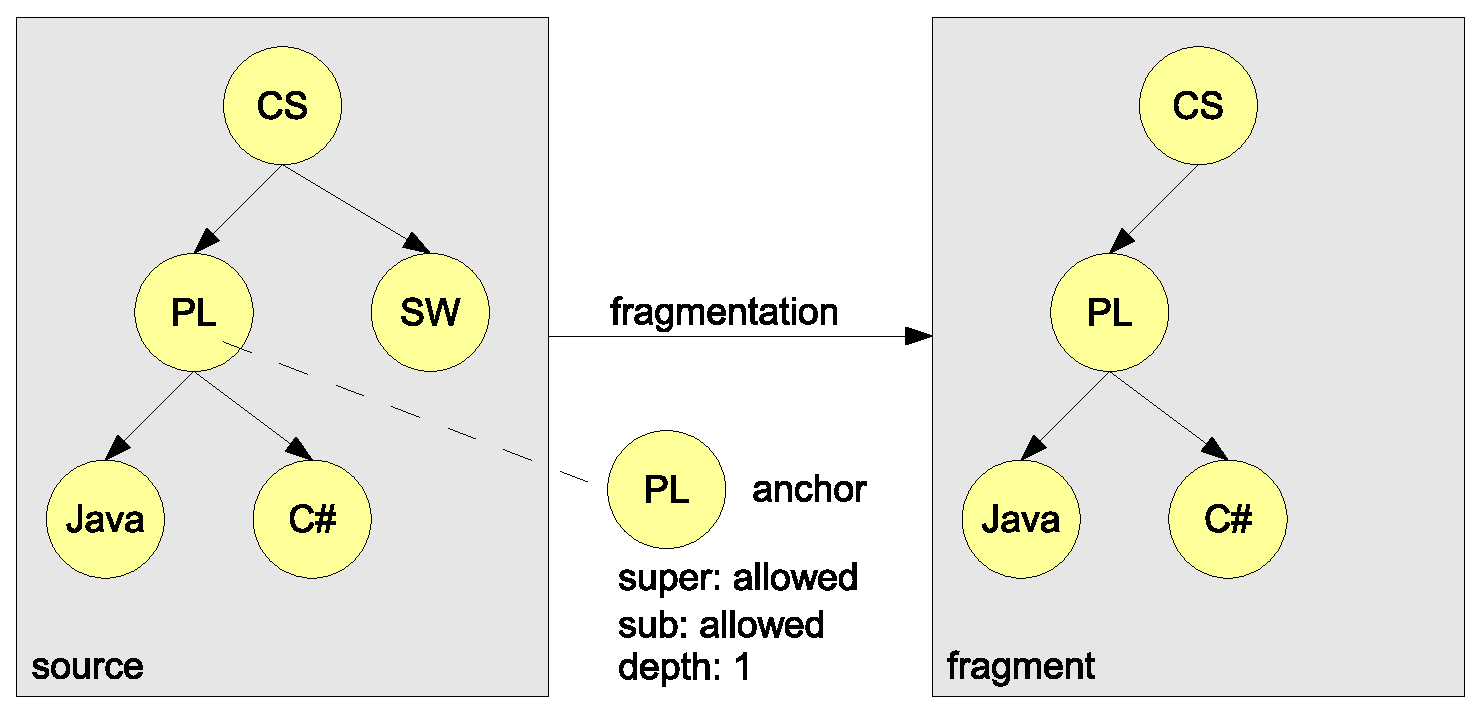
\includegraphics[width=0.60\textwidth]{taxonomyFragmentation.eps}
\caption{Taxonomy fragmentation}
\label{fig:taxonomyFragmentation}
\end{figure}

The following code performs the operation which described in figure \ref{fig:taxonomyFragmentation}.

\begin{verbatim}
Taxonomy txSource = InMemoSharkKB.createInMemoTaxonomy();
TXSemanticTag cs = 
  txSource.createTXSemanticTag("CS", "http://www.cs.de");
TXSemanticTag pl =  
  txSource.createTXSemanticTag("PL", "http://www.pl.de");
TXSemanticTag sw = 
  txSource.createTXSemanticTag("SW", "http://www.sw.de");
TXSemanticTag java = 
  txSource.createTXSemanticTag("Java", "http://www.java.de");
TXSemanticTag csharp =
  txSource.createTXSemanticTag("CSharp", "http://www.csharp.de");

// make pl and sw subtags of cs
pl.move(cs);
sw.move(cs);

// make java and csharp subtags of pl
java.move(pl);
csharp.move(pl);

System.out.println("source:" + L.stSet2String(txSource));

// create anchor tag
SemanticTag anchor = 
  InMemoSharkKB.createInMemoSemanticTag(
    "plAnchor", "http://www.pl.de");

System.out.println("anchor:" + L.semanticTag2String(anchor));

//define fragmentation parameter
boolean superTags = true; // follow super tags
boolean subTags = true; // follow sub tags
int depth = 1; // follow max depth 1

FragmentationParameter fp = 
  new FragmentationParameter(superTags, subTags, depth);

// do fragmentation
STSet fragment = txSource.fragment(anchor, fp);
System.out.println("fragment:" + L.stSet2String(fragment));
\end{verbatim}


\subsection{Semantic net fragmentation}
Fragmentation in semantic networks is the most general variant. It has also a {\tt depth} parameter but instead of two logical values it has two lists of names. They are called {\tt allowedPredicates} and {\tt forbiddenPredicates}. 

Fragmentation in semantic nets is similar to fragmentation in taxonomies except for one variation: The steps three and four in the previous algorithm are replaced with these steps:

All predicates of the current tag are iterated. It is checked for every predicate if it should be used for the fragment. This decision is a little rule-set:

\begin{enumerate}
    \item A predicate is not allowed to follow if its name is in the {\tt forbiddenPredicates} list.

    \item A predicate is not allowed to follow if the {\tt allowedPredicates} list is not empty and the predicate name is not in the list.

\item 
Otherwise the predicate can be used.
\end{enumerate}

Allowed predicates can be followed and all referenced tags are added to the fragment. The previous algorithm is continued with step five.

Figure \ref{fig:semanticNetFragmentation} illustrates a fragmentation with a semantic network. The source contains several relationship between people.

\begin{figure}[t]
\centering
\includegraphics[width=0.60\textwidth]{semanticNetFragmentation.eps}
\caption{Semantic net fragmentation}
\label{fig:semanticNetFragmentation}
\end{figure}

We use Alisha as anchor and allow just the {\it mother} relationship. The depth is set to two. The fragment is just a graph of two concepts: Alisha and her son Ben. Apparently, her sister Carmen isn't reachable by a mother-relation. Therefore, the mother-relationship to Deng isn't part of the fragment.

The following code performs that operation.

\begin{verbatim}

SemanticNet snSource = InMemoSharkKB.createInMemoSemanticNet();
SNSemanticTag alisha, ben, carmen, deng, elias;

alisha = 
  snSource.createSemanticTag("Alisha", "http://www.alisha.de");
ben = 
  snSource.createSemanticTag("Ben", "http://www.ben.de");
carmen = 
  snSource.createSemanticTag("Carmen", "http://www.carmen.de");
deng = 
  snSource.createSemanticTag("Deng", "http://www.deng.de");
elias = 
  snSource.createSemanticTag("Elias", "http://www.elias.de");

// define property names simply as strings
String motherProp = "mother";
String sisterProp = "sister";
String cousinProp = "cousin";
String fatherProp = "father";

// make relations explicit
alisha.setPredicate(sisterProp, carmen);
alisha.setPredicate(motherProp, ben);

carmen.setPredicate(motherProp, deng);

ben.setPredicate(fatherProp, elias);
ben.setPredicate(cousinProp, deng);

System.out.println("source:" + L.stSet2String(snSource));

SemanticTag anchor = 
  InMemoSharkKB.createInMemoSemanticTag(
    "AlishaAnchor", "http://www.alisha.de");

System.out.println("anchor:" + L.semanticTag2String(anchor));

// define allowed properties
Vector<String> allowedProps = new Vector();
allowedProps.add(motherProp);

FragmentationParameter fp = 
    new FragmentationParameter(
            allowedProps, // follow those props
            null, // no forbidden props
            2); // depth == 2

SemanticNet fragment = snSource.fragment(anchor, fp);
System.out.println("fragment:" + L.stSet2String(fragment));
\end{verbatim}

\subsection{Contextualize}
Contextualization is based on fragmentation. There is also a {\it source tag set} of one of our three types. The anchor is no longer a single semantic tag but a semantic tag {\it set}. All other parameters are the same.

{\tt Depth} is used for taxonomies and semantic nets. Both logical values are used for taxonomies and both predicate name lists are used with semantic nets.

The algorithm is short:

\begin{enumerate}

    \item 
An empty tag set is created and called {\it fragment}.
The following step is executed for each tag in the anchor set:

\item
A fragmentation is executed with the source and the current anchor tag and the defined fragmentation parameter. The result is merged into {\it fragment}.

\end{enumerate}
In conclusion, contextualization is a multiple execution of fragmentation.

We use our little family as an example. Figure \ref{fig:semanticnetContextualization} shows the result of a contextualization with the source of figure \ref{fig:semanticNetFragmentation} but Alisha and Carmen as anchor. 

\begin{figure}[t]
\centering
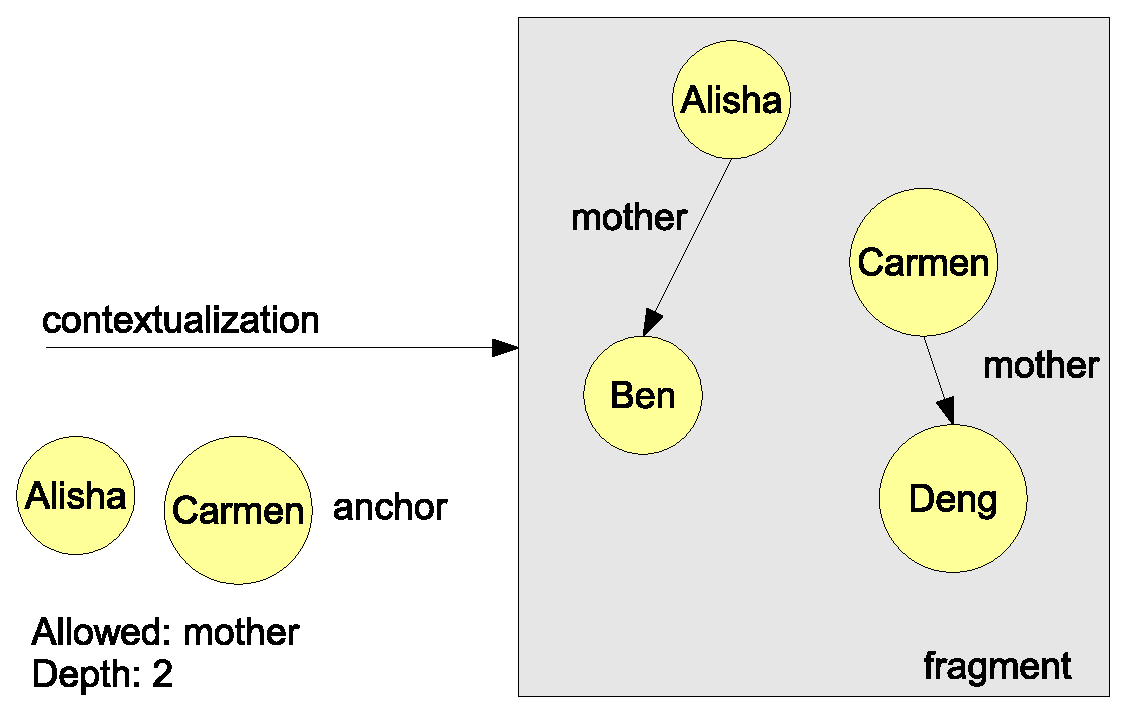
\includegraphics[width=0.60\textwidth]{semanticnetContextualization.eps}
\caption{Semantic net contextualization}
\label{fig:semanticnetContextualization}
\end{figure}

Note: The fragment does not contain relations which are not allowed.
Ben and Deng are part of the fragment. Their relationship is not.
The fact that Carmen is sister of Alisha is also not in the fragment.

For illustration purposes we are going to extend our previous example. 
Let's assume we have still defined Alisha and her family and create an
{\it context} instead of a single anchor:

\begin{verbatim}
STSet context = InMemoSharkKB.createInMemoSTSet();
context.merge(alisha);
context.merge(carmen);

// do contextualization
fragment = snSource.contextualize(context, fp);
System.out.println("after contextualization:" + L.stSet2String(fragment));
\end{verbatim}

Context is an arbitrary tag set. We use the {\tt merge} operation to add tags to the context. Note, merging creates copies of tags in the tag  set. Contextualization differs just in a single parameter from fragmentation.

\section{PeerSNSemanticTag and friends}
We have now discussed Semantic Tags and tag sets. We have learned about special Semantic Tags like Peer Semantic Tags. We have worked with special tag sets, namely taxonomies and semantic nets. 

\begin{figure}[t]
\centering
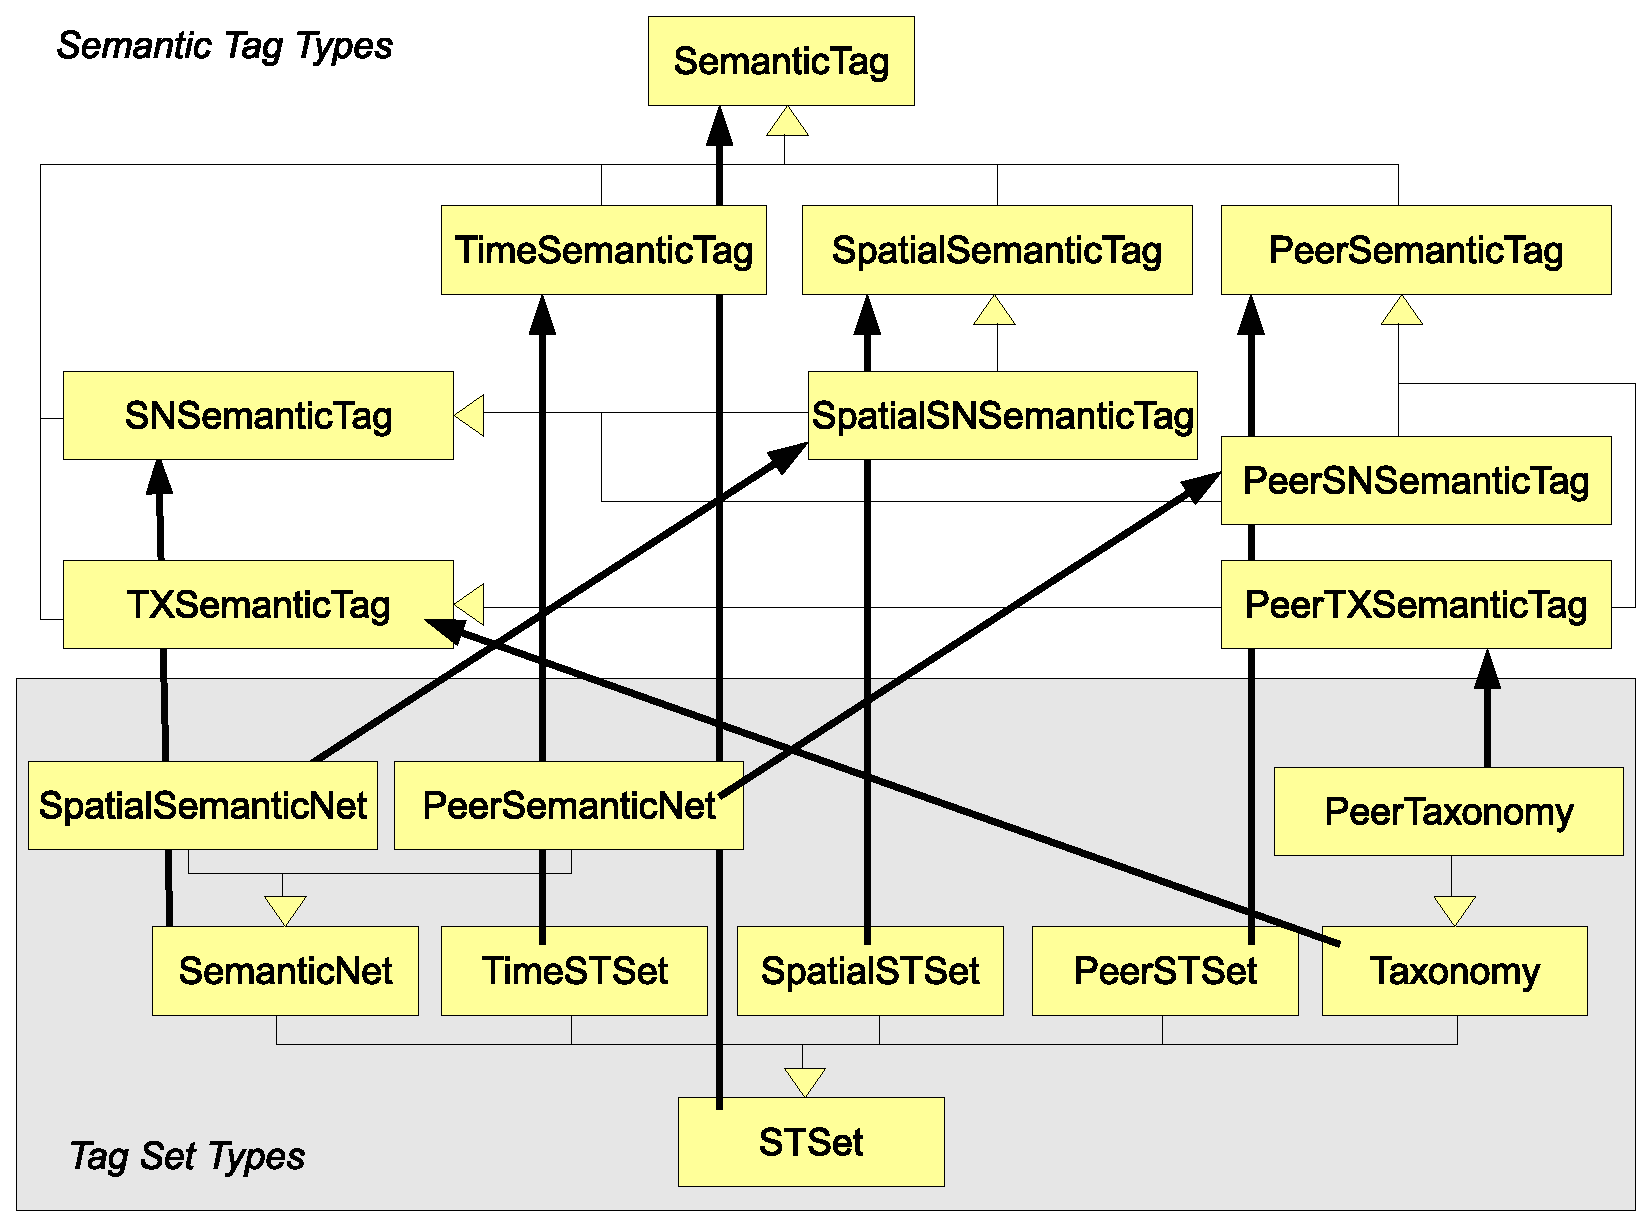
\includegraphics[width=0.80\textwidth]{tagsSetTypes.eps}
\caption{Semantic Tag and tag set types}
\label{fig:tagsSetTypes}
\end{figure}

Apparently, a peer semantic tag {\it is a} semantic tag. That fact can be coded with Java by deriving the {\tt PeerSemanticTag} from {\tt SemanticTag}.  Actually, it is the first line of code in the {\tt PeerSemanticTag} interface:

\begin{verbatim}
public interface PeerSemanticTag extends SemanticTag {..}
\end{verbatim}

There is a similar situation with sets. The most general tag set is {\tt STSet}. Two interfaces extend its abilities: {\tt Taxonomy} and {\tt SemanticNet}:

\begin{verbatim}
public interface SemanticNet extends STSet {..}
public interface Taxonomy extends STSet {..}
\end{verbatim}

Each tag set allows accessing Semantic Tags. For example, one get method declaration is this:

\begin{verbatim}
public SemanticTag getSemanticTag(String si) 
     throws SharkKBException;
\end{verbatim}

There are sets which only contain {\tt PeerSemanticTags}. We have declared a {\tt PeerSTSet} to be type safe in Java. It extends {\tt STSet} and offers a special get method:

\begin{verbatim}
public PeerSemanticTag getSemanticTag(String si) 
     throws SharkKBException;
\end{verbatim}

Note, method name is identical but return type has changed from {\tt SemanticTag} to {\tt PeerSemanticTag}.

Now it becomes a bit complicated due to possible combinations. Just relax and read the following comments calmly. 

There can be a taxonomy that contains Peer Semantic Tags. That set (interface) is declared as {\tt PeerTaxonomy} which extends Taxonomy. It offers a method:

\begin{verbatim}
public PeerTXSemanticTag getSemanticTag(String[] sis) 
     throws SharkKBException;
\end{verbatim}

Have a look at the return type. It is a {\tt PeerTXSemanticTag} which declares a Peer Semantic Tag that is stored in a taxonomy. Such a tag can be handled as Peer Semantic Tag. Addresses can be set for instance. It can also be handled as member of a taxonomy. It can be moved in the tag hierarchy.

There is a number of such combinations, e.g.

\begin{description}
\item[PeerSNSemanticTag] which is a Peer Semantic Tag in a semantic net.
\item[SNSemanticTag] which is general Semantic Tag in a semantic net.
\item[TXSemanticTag] which is general Semantic Tag in a taxonomy.
\item[SpatialSNSemanticTag] which is general Spatial Semantic Tag in a semantic net.
\end{description}

Such types inherit features from two interfaces. Here is an example:
\begin{verbatim}
public interface PeerTXSemanticTag 
     extends TXSemanticTag, PeerSemanticTag {}
\end{verbatim}
No further methods are declared. It is just an aggregation of two existing interfaces, {\tt TXSemanticTag} and {\tt PeerSemanticTag} in this case.


Figures \ref{fig:tagsSetTypes} illustrates that interface hierarchy. The most general semantic tag is to been seen on top the diagram. It has five sub types (spatial, time, peer and taxonomy and semantic net tags). There are three combinations which inherit from two interfaces 
({\tt SpatialSNSemanticTag}, {\tt PeerSNSemanticTag} and 
{\tt PeerSNSemanticTag}.

The tags set hierarchy starts with its most general concept on the bottom ({\tt STSet}. It has two sub types by structure: ({\tt Taxonomy} and {\tt SemanticNet} and three sub types by content types: {\tt PeerSTSet}, {\tt SpatialSTSet} and {\tt TimeSTSet}. Taxonomies and semantic nets can have more specific sub types, namely semantic nets or taxonomies which contain peers ({\tt PeerSemanticNet}, {\tt PeerTaxonomy}). There is also a {\tt SpatialSemanticNet} to describe a network of geographically referenced objects. Other possible combinations like networks of time tags do not exist. There wasn't a need for such combinations until now.

The thick arrows describes a usage relations. A {\tt PeerSemanticNet} e.g. uses (or contains) objects of type {\tt PeerSNSemanticTag}. The most general {\tt STSet} stores {\tt SemanticTag} objects etc.

Why dealing with that mess? Because of types! Type safe programming is professional programming. Thus, peer information have to be stored in a {\tt PeerSTSet} and not in a general {\tt STSet}. In most cases, programmers aren't bothered with choosing the right tags set type. And that is good news. Usually it is already dictated by the knowledge base and its underlying concept of context space which will be described in the next chapter.

\section{Exercises}
\begin{enumerate}
\item 
Change the code from section \ref{sec:taxonomyFragmentation} and let sister relations become part of the fragment.
\item 
\item 

\end{enumerate}
